\documentclass[11pt]{article}
\usepackage[margin=0.88in]{geometry}
\usepackage[T1]{fontenc}
\usepackage{lmodern}
\usepackage{microtype}
\usepackage{amsmath,amssymb,amsthm,mathtools}
\usepackage{graphicx}
\usepackage{booktabs,tabularx,array,longtable,multirow}
\usepackage{float}
\usepackage{xcolor}
\usepackage{hyperref}
\usepackage[backend=biber,style=authoryear,maxbibnames=6]{biblatex}
\addbibresource{paper.bib}
\hypersetup{colorlinks=true,linkcolor=blue!45!black,citecolor=blue!45!black,urlcolor=blue!45!black,pdftitle={Two Information Channels, One Design Limit: An Information-Theoretic Framework for Generative AI in Synthetic Gene-Circuit Design},pdfauthor={Devanik Debnath}}
\graphicspath{{figures/}}
\setlength{\parskip}{0.35em}
\setlength{\parindent}{1.1em}
\renewcommand{\arraystretch}{1.12}
\setcounter{topnumber}{4}\setcounter{bottomnumber}{3}\setcounter{totalnumber}{6}
\setcounter{secnumdepth}{3}
\newtheorem{proposition}{Proposition}
\newtheorem{corollary}{Corollary}
\newtheorem{definition}{Definition}
\newcommand{\I}{\mathrm{I}}
\newcommand{\Hh}{\mathrm{H}}
\newcommand{\Pp}{\mathbb{P}}
\newcommand{\E}{\mathbb{E}}
\newcommand{\KL}{D_{\mathrm{KL}}}
\newcommand{\bits}{\,\mathrm{bits}}
\title{\textbf{Two Information Channels, One Design Limit:}\\[0.25em]\large An Information-Theoretic Framework for Generative AI in Synthetic Gene-Circuit Design}
\author{Devanik Debnath\\
\small Electronics and Communication Engineering, National Institute of Technology Agartala, India\\
\small ORCID: \href{https://orcid.org/0009-0001-8310-6921}{0009-0001-8310-6921}\\[0.4em]
\small Research-process orchestration: Xylia}
\date{17 October 2026\\[0.35em]\small Theoretical preprint; not peer reviewed}
\begin{document}
\maketitle
\begin{abstract}
Generative models can propose candidate genetic circuits, but generation quality is not the same as reliable function after a circuit is realized in a particular biological context. We formulate this gap as a composition of two information channels: a proposal channel from a desired functional class to a generated design, and a realization channel from that design to its context-dependent phenotype. Under an explicit conditional Markov assumption, the data-processing inequality bounds target-relevant information in realized phenotypes by the information retained in generated designs and by the capacity of the realization channel. For idealized $K$-ary symmetric channels, we derive the composed mismatch rate and its capacity, then evaluate the consequences in a reproducible synthetic sensitivity analysis. With illustrative (not measured) error rates of 0.10 at proposal and 0.15 at realization, a four-class symmetric-channel example yields a composed mismatch of 0.23 and an effective channel capacity of approximately 0.86 bits per use, below either stage's capacity. The result is a framework, not a claim about any specific model, circuit, organism, or wet-lab performance. Four plots, two dependency graphs, two workflow diagrams, and six tables expose assumptions, composition rules, finite-sample uncertainty, and falsification requirements. The practical implication is methodological: generative candidates should be evaluated with calibrated, context-stratified, independent functional validation, and claims should be bounded by the weakest characterized link in the chain. The paper contributes a formal decomposition and a reproducible null model intended to guide evaluation design; empirical calibration is left for future work.
\end{abstract}

\noindent\textbf{Keywords:} synthetic biology; generative models; information theory; gene regulatory circuits; data-processing inequality; channel capacity; uncertainty quantification; context shift

\section{Research question and contribution}
Synthetic gene circuits combine regulatory components into systems intended to implement a target response, such as a switch, oscillator, or adaptive response. Their behavior depends on component interactions, context, resource competition, noise, and construction choices; even established design principles identify substantial failure modes in composition and in-vivo operation \parencite{Elowitz2000,Gardner2000,BrophyVoigt2014}. In parallel, machine-learning models have been explored for circuit design and for ranking biological parts. A recent study used a conditional variational autoencoder to propose RNA-circuit topologies with desired dynamical and evolutionary properties in an in-silico environment \parencite{GallupSteel2026}. That result is important evidence that the generative-design question is now concrete; it does not remove the distinction between generated structure, predicted function, and realized phenotype.

The question here is narrower than whether generative AI can design a circuit: \emph{what information-theoretic limits apply when a desired functional specification is transformed into a model-generated design and then into a context-dependent realized phenotype?} The analysis does not assume that present systems have a known error rate, nor does it estimate one from public data. Instead, it gives explicit conditional bounds and a synthetic testbed that makes their assumptions inspectable.

The contribution has four parts. First, we define a two-channel abstraction that separates proposal error from biological realization error. Second, we derive the data-processing and symmetric-channel consequences, including a closed-form composition rule. Third, we implement a small reproducible analysis showing how information can be lost across stages and how finite sample size affects estimates. Fourth, we give a validation design that separates predictive calibration, context robustness, functional validation, and empirical realization. This is a theory-and-methods preprint; it reports no new biological experiments, no sequence-level gene-circuit designs, and no clinically actionable construct.

\section{Scope and epistemic posture}
The model is intended for evaluation architecture, not for predicting the behavior of a named construct. Circuit function is represented by a finite set of functional classes only to make the channel derivations transparent. Real circuit functions may be continuous, multi-objective, partially observed, and dependent on environmental covariates. Discretization is therefore an analytical convenience whose validity must be tested for any application.

\begin{table}[H]
\centering\small
\caption{Epistemic status of the paper's main elements.}
\begin{tabularx}{\linewidth}{p{0.18\linewidth} X p{0.20\linewidth}}
\toprule
Element & Statement & Status \\
\midrule
Data-processing inequality & Information cannot increase along the stated Markov chain. & Exact theorem under assumptions \\
$K$-ary symmetric channel & Closed-form capacity and composition are derived from the channel definition. & Exact model result \\
Illustrative mismatch rates & Stage errors 0.10 and 0.15 are used to demonstrate arithmetic. & Hypothetical, not measured \\
Context-shift curve & Errors increase linearly with a normalized shift parameter by construction. & Sensitivity scenario only \\
Deployment implications & Independent validation and context-stratified testing can reveal model failures. & Methodological recommendation \\
Biological efficacy & No inference about a real circuit's efficacy, safety, or performance is made. & Untested / out of scope \\
\bottomrule
\end{tabularx}
\end{table}

In the P1--P5 hierarchy, the inequalities and channel identities below are P1 mathematical consequences. The use of symmetric channels as approximations is a P4 modelling correspondence. The assumed dependence of error on normalized context shift is P5 illustrative intuition made numerically explicit, not an empirical law. The framework does not promote the latter two categories into measured mechanisms.

\section{Related work and the gap addressed}
Information theory has long been used to characterize limits of communication and regulatory systems, beginning with foundational channel-capacity theory \parencite{Shannon1948}. Tka\v{c}ik, Callan, and Bialek formalized the information capacity of genetic regulatory elements under physically motivated noise and showed that the answer depends on the input distribution and noise model \parencite{Tkacik2008}. Their capacity concerns signal transmission through gene regulation, whereas the present abstraction adds a separate model-proposal channel upstream of biological realization. The two settings are compatible but not interchangeable.

Classic synthetic circuits established that compact regulatory networks can implement designed behaviors, including a repressilator and a bistable toggle switch \parencite{Elowitz2000,Gardner2000}. Reviews emphasize context dependence, part interactions, resource constraints, and design failure modes \parencite{BrophyVoigt2014,Wall2004}. A broad review also organizes circuit-design approaches from brute-force searches through control-theoretic formulations and emphasizes that objective definitions and robustness strategies matter \parencite{Chakraborty2022}. These studies motivate treating realized function as a channel with uncertainty rather than assuming deterministic execution of a design.

The closest direct antecedent is Gallup and Steel (2026), who generated RNA-circuit topologies for target dynamics using in-silico simulation and examined functional and evolutionary properties \parencite{GallupSteel2026}. Their result shows both capability and challenges: generated output must be simulated to assess prompt adherence, performance depends on objective representation, and a simulated circuit is not automatically an experimental result. Our paper does not reproduce or outperform their method. Instead, it asks how to reason about the combined ceiling implied by the proposal and realization channels, independently of a particular generative architecture.

\begin{table}[H]
\centering\small
\caption{Selected prior work and the specific boundary it informs.}
\begin{tabularx}{\linewidth}{p{0.22\linewidth} X X}
\toprule
Work & Established contribution relevant here & Boundary relative to this paper \\
\midrule
Tka\v{c}ik et al. (2008) & Information capacity of noisy gene-regulatory elements. & Does not explicitly factor an AI proposal stage. \\
Elowitz and Leibler (2000) & Synthetic genetic oscillator (repressilator). & Demonstrates circuit construction, not a universal AI design bound. \\
Gardner et al. (2000) & Genetic toggle switch and bistability. & Demonstrates engineered behavior, not generative-model calibration. \\
Brophy and Voigt (2014) & Circuit design principles and failure modes. & Supplies biological context, not the composed-channel formulation. \\
Chakraborty, Rengaswamy, and Raman (2022 review) & Organizes circuit design methods and robustness concerns. & Does not provide the present two-stage capacity comparison. \\
Gallup and Steel (2026) & Generative circuit-topology design with simulated functional/evolutionary objectives. & Closest generative precedent; motivates a cross-stage limit, not a novelty claim about generation. \\
\bottomrule
\end{tabularx}
\end{table}

The literature reviewed supports a precise gap statement: despite substantial work on noisy regulatory information and emerging generative circuit design, this paper has not found a standard, explicit two-stage channel decomposition used as a generic release-time audit for proposal uncertainty and context-conditioned functional realization. This is a scoped statement about the searched sources, not a claim of absolute priority. A broader search could reveal equivalent decompositions under different terminology; the mathematical ingredients themselves are established.

\section{Model and assumptions}
Let $T\in\mathcal{T}$ denote a desired functional class, where $|\mathcal{T}|=K\geq2$. Let $D$ denote model training/evaluation evidence, $G$ a generated design representation, $C$ a biological context (for example, host background or operating environment), $Y$ the realized functional class, and $A$ the assay result. The graph in Figure~\ref{fig:channelgraph} records this abstraction and possible evidence dependencies.

We assume that, conditional on context $C$, the functional path is Markov:
\begin{equation}
T \longrightarrow G \longrightarrow Y \longrightarrow A,
\label{eq:markov}
\end{equation}
where the arrows encode conditional dependencies, not time alone. Training evidence and model choice affect the proposal distribution; context and unmodeled interactions can affect realization; assay noise affects observation. If the chain does not adequately represent a particular application—for example, if the assay itself influences the realized phenotype or the proposed design bypasses a stage—the bound must be reformulated.

\begin{table}[H]
\centering\small
\caption{Notation and operational interpretation.}
\begin{tabularx}{\linewidth}{p{0.14\linewidth} p{0.24\linewidth} X}
\toprule
Symbol & Meaning & Required operationalization in an application \\
\midrule
$T$ & Target function class & Predeclared phenotype label or target region \\
$G$ & Generated design & Representation actually passed to independent evaluation \\
$Y$ & Realized function & Measured or independently simulated phenotype under context $C$ \\
$C$ & Context & Host, environment, growth state, or other effect modifier \\
$A$ & Assay observation & Measurement with a declared noise/error model \\
$e_g$ & Proposal-stage mismatch & Estimated on held-out, leakage-controlled targets \\
$e_b$ & Realization-stage mismatch & Estimated under context-stratified independent validation \\
$K$ & Number of functional classes & Fixed before evaluation; class imbalance reported \\
$I(X;Y)$ & Mutual information & Calculated from a validated joint distribution, with uncertainty \\
\bottomrule
\end{tabularx}
\end{table}

\subsection{Information ceiling from data processing}
Conditional on $C$, the data-processing inequality gives
\begin{equation}
\I(T;Y\mid C) \leq \I(T;G\mid C).
\label{eq:dpi}
\end{equation}
If measurement is another downstream stochastic transformation, then
\begin{equation}
\I(T;A\mid C) \leq \I(T;Y\mid C) \leq \I(T;G\mid C).
\label{eq:dpi_assay}
\end{equation}
These bounds do not say that $G$ always contains useful information, nor that $I(T;G)$ can be estimated from a language-model confidence score. They say that downstream stochastic stages cannot recover target-relevant information that earlier stages have already lost, under the stated dependency assumptions. Side information, feedback, active experimental design, or adaptive retraining changes the graph and may improve later cycles; it does not invalidate the single-cycle inequality when correctly conditioned.

Suppose the realization channel $P(Y\mid G,C=c)$ has capacity $C_{\mathrm{bio}}(c)=\max_{P(G)} I(G;Y\mid C=c)$. Then
\begin{equation}
\I(T;Y\mid C=c) \leq \min\{\I(T;G\mid C=c),\ C_{\mathrm{bio}}(c)\}.
\label{eq:minbound}
\end{equation}
The first term is limited by what the proposal process preserved about the target; the second by the information that the realization channel can transmit for the chosen representation and context. These are separate estimands and need separate evidence. If target labels are imbalanced, the achieved mutual information and optimal channel input distribution may differ from capacity.

\subsection{A tractable categorical model}
For a transparent sensitivity analysis, assume each stage is a $K$-ary symmetric channel. At either stage the correct class occurs with probability $1-e$ and each of the other $K-1$ classes occurs with probability $e/(K-1)$. Such a channel is deliberately restrictive: it has uniform error across wrong classes and excludes class-specific failure modes.

\begin{definition}[Symmetric channel capacity]
For a $K$-ary symmetric channel with mismatch probability $e\in[0,1-1/K]$, its capacity under the symmetric-channel model is
\begin{equation}
C_K(e)=\log_2 K-H_2(e)-e\log_2(K-1),
\label{eq:capacity}
\end{equation}
where $H_2(e)=-e\log_2 e-(1-e)\log_2(1-e)$ with endpoint terms defined by continuity.
\end{definition}

Now let proposal and realization errors be $e_g$ and $e_b$ and assume the two stage transitions are conditionally independent given their input class. The final class is correct when both stages are correct, or when an intermediate error lands on the final target class. Therefore
\begin{equation}
1-e_{\mathrm{tot}}=(1-e_g)(1-e_b)+\frac{e_g e_b}{K-1},
\label{eq:composition_correct}
\end{equation}
and equivalently
\begin{equation}
e_{\mathrm{tot}}=e_g+e_b-\frac{K}{K-1}e_g e_b.
\label{eq:composition_error}
\end{equation}
The correction term accounts for error cancellation in the symmetric model. It should not be interpreted as a general law of biology: class-dependent errors, correlated stages, context mixtures, or multi-objective outcomes require the full transition matrices rather than two scalar error rates.

\begin{proposition}[Composed symmetric-channel bound]
Under the conditional Markov and independent symmetric-channel assumptions, with uniform target classes, the end-to-end capacity is $C_K(e_{\mathrm{tot}})$ and does not exceed either stage capacity when each stage operates in its nonnegative-capacity range.
\end{proposition}
\begin{proof}
Composition of two symmetric transition matrices is again symmetric, with mismatch in Equation~\eqref{eq:composition_error}. Its capacity follows from Equation~\eqref{eq:capacity}. The information ceiling follows independently from the data-processing inequality in Equation~\eqref{eq:dpi} applied in both directions along $T\to G\to Y$; the exact numerical gap is model-dependent.
\end{proof}

\begin{table}[H]
\centering\small
\caption{Mathematical claims and the assumptions they require.}
\begin{tabularx}{\linewidth}{p{0.23\linewidth} X X}
\toprule
Claim & Assumptions & What it does not establish \\
\midrule
$I(T;Y\mid C)\leq I(T;G\mid C)$ & $T\to G\to Y$ is Markov after conditioning on context. & A numerical value for real-model performance. \\
$C_K(e)$ expression & $K$-ary symmetric channel; uniform optimum; $e\leq1-1/K$. & Capacity of a specific biological circuit. \\
Error composition & Independent symmetric stage transitions with same $K$. & Correctness under correlated or class-dependent errors. \\
Context sensitivity curve & Declared hypothetical map from shift to error. & A measured context law or biological mechanism. \\
Finite-sample interval plot & Binomial observations at an assumed fixed error. & Calibration, model bias, or experimental sample requirements. \\
\bottomrule
\end{tabularx}
\end{table}

\section{Reproducible synthetic analysis}
The implementation in \texttt{verify\_model.py} provides independent functions for binary entropy, symmetric-channel capacity, error composition, stochastic-channel construction, and mutual information. The script uses NumPy and Matplotlib plus NetworkX for graph-structured schematics. The random seed is 20261017; randomness appears only in a binomial illustration. It regenerates four plots, two dependency graphs, two flow diagrams, a table of plotted numerical outputs, a JSON summary, and a machine-readable verification report. No biological sequences, organisms, laboratory protocols, or measured phenotypes are simulated.

\subsection{Scenario and numerical illustration}
For $K=4$, $e_g=0.10$, and $e_b=0.15$, Equation~\eqref{eq:composition_error} yields $e_{\mathrm{tot}}=0.23$. Applying Equation~\eqref{eq:capacity} gives stage capacities of approximately 1.37 bits/use and 1.15 bits/use and a composed capacity of approximately 0.86 bits/use. The precise values are computed and archived by the released script. This is not an estimate of a biological circuit's error; it only illustrates that two nonzero mismatch stages can create an end-to-end channel with less capacity than either component.

\begin{table}[H]
\centering\small
\caption{Analytical/synthetic illustration reported by the current code run. Values are assumptions, not biological measurements.}
\begin{tabular}{lrr}
\toprule
Quantity & $K=4$ example & Units \\
\midrule
Assumed proposal mismatch $e_g$ & 0.100 & probability \\
Assumed realization mismatch $e_b$ & 0.150 & probability \\
Composed mismatch $e_{\mathrm{tot}}$ & 0.230 & probability \\
Proposal-stage capacity $C_4(e_g)$ & 1.37 (approx.) & bits/use \\
Realization-stage capacity $C_4(e_b)$ & 1.15 (approx.) & bits/use \\
Composed capacity $C_4(e_{\mathrm{tot}})$ & 0.86 (approx.) & bits/use \\
\bottomrule
\end{tabular}
\end{table}

\begin{figure}[H]
\centering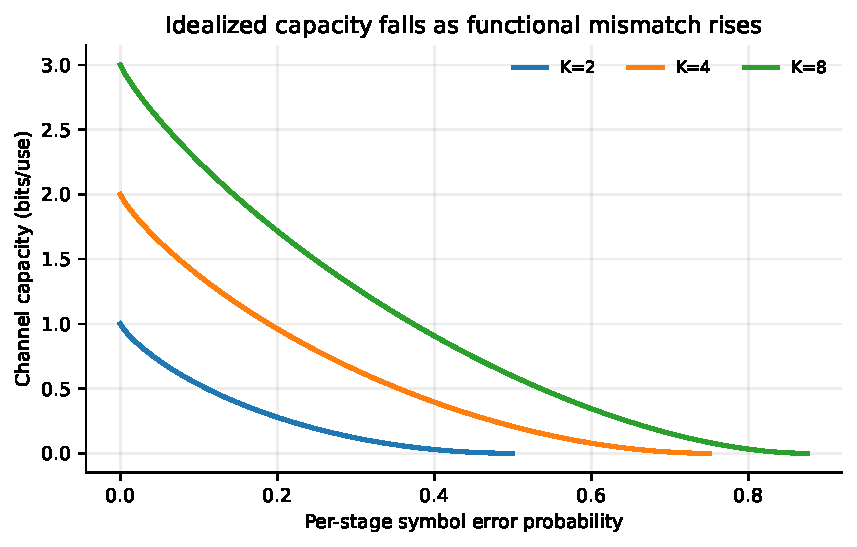
\includegraphics[width=.88\linewidth]{figure01_capacity_vs_error.pdf}
\caption{Channel capacity as a function of mismatch for $K\in\{2,4,8\}$. Curves are exact evaluations of the stated symmetric-channel formula, not fitted biological curves.}
\label{fig:capacity}
\end{figure}

\begin{figure}[H]
\centering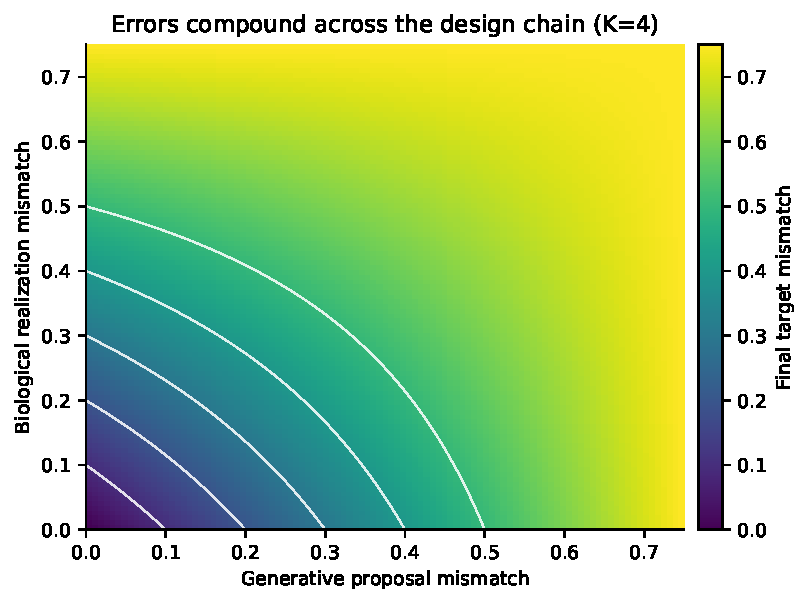
\includegraphics[width=.86\linewidth]{figure02_composed_error_heatmap.pdf}
\caption{Composed mismatch for a four-class symmetric channel across proposal- and realization-stage errors. Both axes are sensitivity parameters; the plotted surface is model-generated.}
\label{fig:heatmap}
\end{figure}

Figure~\ref{fig:capacity} illustrates the channel's loss of distinguishable classes as mismatch approaches random guessing. Figure~\ref{fig:heatmap} makes the two-stage dependence explicit and avoids collapsing the model into a single generative score. In actual evaluation, the two axes should be replaced with separately estimated, uncertainty-bearing quantities and should be stratified by relevant context rather than pooled without analysis.

\subsection{Context shift and finite-sample uncertainty}
To demonstrate sensitivity to distribution shift, the code uses normalized shift $s\in[0,1]$ and assigns hypothetical proposal and realization mismatch rates $e_g(s)=0.04+0.22s$ and $e_b(s)=0.06+0.24s$. These linear functions were selected for illustration only. The resulting curve in Figure~\ref{fig:shift} shows the arithmetic consequences of the assumptions, not how a particular promoter, host, or model behaves. The graph should be read as a stress-test template: an application must estimate the shift-response relationship from held-out environments or state it as unknown.

\begin{figure}[H]
\centering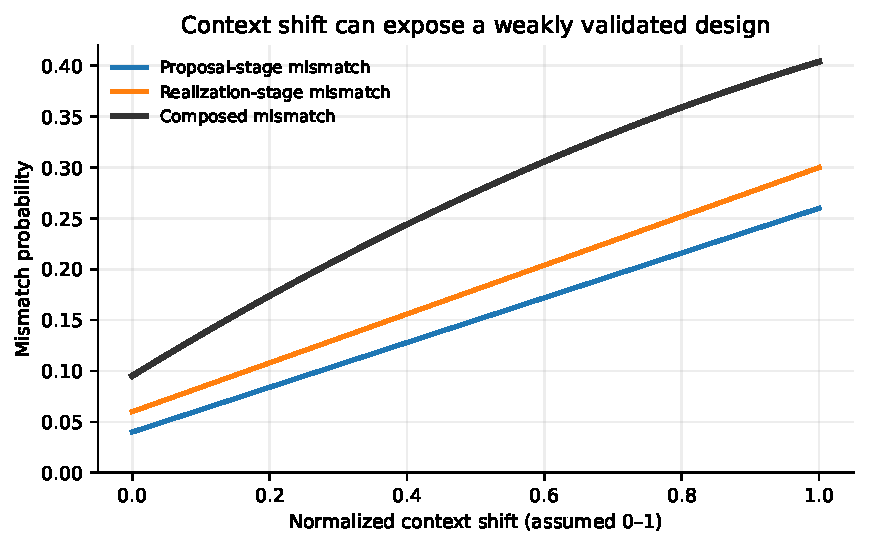
\includegraphics[width=.88\linewidth]{figure03_context_shift.pdf}
\caption{Hypothetical context-shift sensitivity. Linear stage-error functions are assumptions chosen to illustrate composition; no empirical context-shift data are used.}
\label{fig:shift}
\end{figure}

The fourth plot fixes an illustrative mismatch probability at 0.15 and simulates independent Bernoulli observations for sample sizes between 20 and 1280, using 1500 Monte Carlo replicates per sample size. Figure~\ref{fig:sample} shows the empirical distribution's 2.5th and 97.5th percentiles. Increasing sample size narrows sampling variability under the binomial assumption, but does not repair distribution shift, label leakage, a misspecified class set, assay bias, or dependence among replicates. Replication at the wrong abstraction level can give tight but misleading intervals.

\begin{figure}[H]
\centering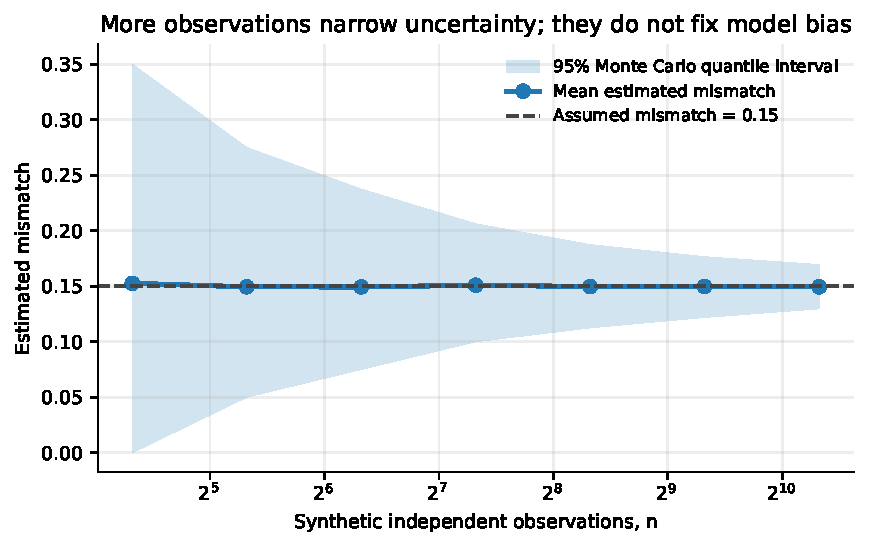
\includegraphics[width=.88\linewidth]{figure04_finite_sample_uncertainty.pdf}
\caption{Monte Carlo uncertainty of an estimated mismatch rate under a synthetic binomial model with assumed true error 0.15. Bands are quantiles across simulation replicates, not confidence intervals from experimental measurements.}
\label{fig:sample}
\end{figure}

\begin{table}[H]
\centering\small
\caption{Reproducibility parameters and what they support.}
\begin{tabularx}{\linewidth}{p{0.25\linewidth} p{0.25\linewidth} X}
\toprule
Parameter / artifact & Current value & Interpretation \\
\midrule
Pseudo-random seed & 20261017 & Reproducible synthetic binomial sample \\
Functional classes & $K=2,4,8$ for capacity plot & Generic discrete labels, not circuit types \\
Finite-sample scenario & $e=0.15$, 1500 replicates & Precision illustration only \\
Context-shift scenario & $e_g=0.04+0.22s$, $e_b=0.06+0.24s$ & User-replaceable sensitivity assumption \\
Data export & \path{results/model_outputs.csv} & Values underlying plotted curves and grid samples \\
Machine report & \path{results/verification_report.json} & Actual run status, tests, environment \\
\bottomrule
\end{tabularx}
\end{table}

\section{Architecture graphs: hidden dependencies and context}
The first graph in Figure~\ref{fig:channelgraph} marks a proposal channel from the desired class to the generated design and a realization channel to the phenotype; context and assay conditions are explicit covariates. The second graph (Figure~\ref{fig:depgraph}) shows dependency paths that can make a model's reported score look better than end-to-end function. For example, if training support is tied to familiar prompt patterns, or if context affects both the observed training data and measured phenotype, a random split may not estimate performance under a new context. The graph is a causal hypothesis template, not a validated causal graph for every circuit.

\begin{figure}[H]
\centering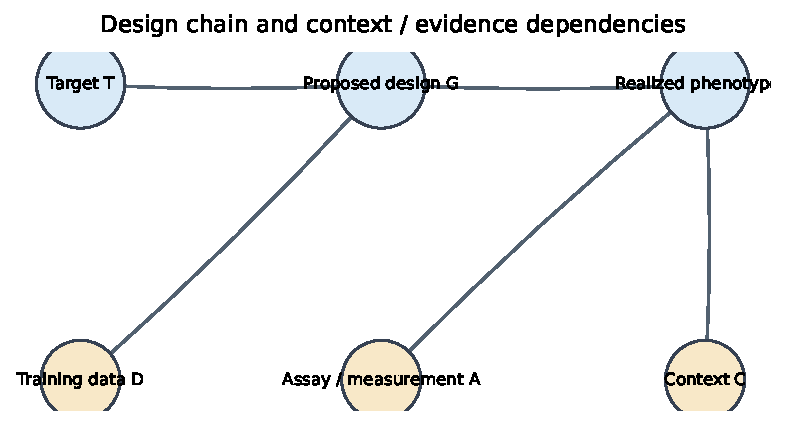
\includegraphics[width=.9\linewidth]{figure05_design_channel_graph.pdf}
\caption{Dependency graph for target, generated design, realized phenotype, context, training support, and assay. Arrows denote candidate conditional dependencies in the abstraction; they are not measured causal effects.}
\label{fig:channelgraph}
\end{figure}

\begin{figure}[H]
\centering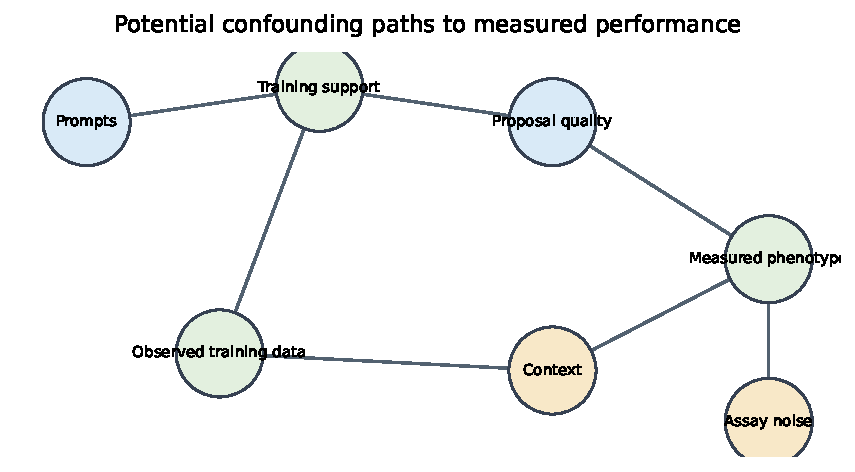
\includegraphics[width=.98\linewidth]{figure06_context_dependency_graph.pdf}
\caption{Potential dependencies that can confound reported model performance. This is a schematic for evaluation planning, not a data-derived graph.}
\label{fig:depgraph}
\end{figure}

The key operational issue is that generative diversity and target adherence are different. A proposal distribution can be diverse while missing its target; it can also produce many near-duplicates with superficially high scores. Similarly, a simulator can score a design against the same assumptions that generated it, yielding an optimistic internal measure. Independent scoring, held-out contexts, counterfactual comparisons, calibration checks, and explicit abstention criteria help distinguish these situations. They do not guarantee success, and their value depends on whether the holdout actually represents the deployment context.

\section{Validation and falsification protocol}
A useful framework should be capable of being rejected or narrowed. The proposed release-time validation sequence appears in Figure~\ref{fig:pipeline}. The second diagram (Figure~\ref{fig:gate}) explicitly permits revision or abstention: a failed uncertainty or robustness gate is an outcome, not a reason to lower a threshold silently.

\begin{figure}[H]
\centering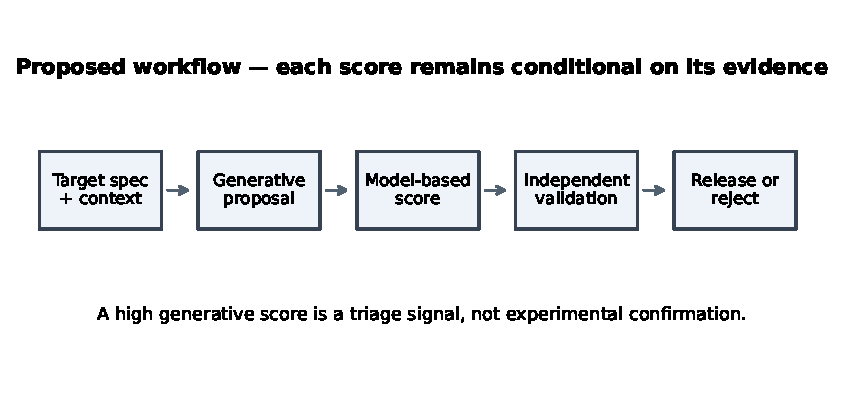
\includegraphics[width=.97\linewidth]{figure07_validation_pipeline_flow.pdf}
\caption{Proposed evaluation pipeline from a predeclared target to independent validation and a release/reject decision. It is a methodological proposal, not an executed wet-lab pipeline.}
\label{fig:pipeline}
\end{figure}

\begin{figure}[H]
\centering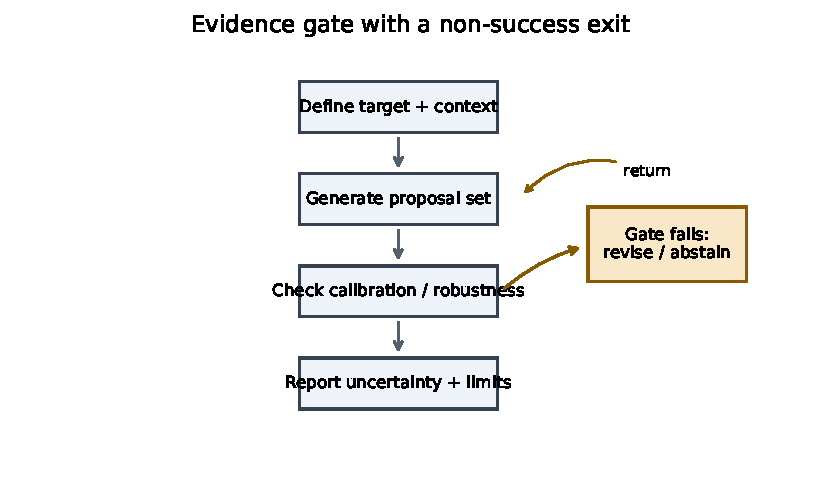
\includegraphics[width=.92\linewidth]{figure08_evidence_gate_flow.pdf}
\caption{Evidence gate with a non-success path. A proposal failing calibration, robustness, or evidence sufficiency should be revised or withheld rather than represented as validated.}
\label{fig:gate}
\end{figure}

\begin{table}[H]
\centering\small
\caption{Predeclared falsification and failure criteria for an empirical follow-up.}
\begin{tabularx}{\linewidth}{p{0.22\linewidth} X X}
\toprule
Claim under test & Falsifying observation / failure criterion & Interpretive consequence \\
\midrule
The proposal channel carries target information & On a leakage-controlled held-out set, target-conditioned outputs are indistinguishable from target-shuffled controls within uncertainty. & Do not claim useful target conditioning for that task. \\
The model's uncertainty is calibrated & Predicted confidence systematically fails to match held-out frequencies or the calibration gap exceeds a preregistered threshold. & Do not use confidence as a proxy for functional reliability. \\
A proposed circuit transfers across contexts & Performance degrades beyond a preregistered tolerance in held-out contexts. & Restrict the claim to evaluated contexts; retraining may be needed. \\
The realization channel is adequately captured by a scalar $e_b$ & Errors differ substantially by class/context or errors are correlated across stages. & Replace the symmetric scalar model with transition matrices or a richer model. \\
Observed gains reflect generation rather than scoring leakage & Gains disappear under an independent evaluator or deduplicated test set. & Treat prior score as an evaluator artifact, not functional design progress. \\
\bottomrule
\end{tabularx}
\end{table}

A credible empirical study should predeclare (i) target classes or continuous objectives; (ii) the independent unit of split; (iii) calibration metrics and acceptable error; (iv) the relevant context distribution; (v) the exact proposal and realization endpoints; (vi) how failed designs, missing outcomes, and inconclusive outcomes are counted; and (vii) what change would falsify the intended claim. The model should be compared with simple non-generative baselines, existing circuit-design methods, and random or target-shuffled controls where meaningful. If only simulated ground truth is available, results must be described as simulator-conditional.

\section{Limitations and alternative explanations}
The most important limitation is abstraction. A $K$-ary symmetric channel makes mistakes equally likely across the $K-1$ incorrect classes. Genetic circuits rarely satisfy this assumption automatically: some phenotypes may be much more likely than others, several functional modes may be close in measurement space, and errors may correlate across design generation, prediction, host context, and assay. The exact formula in Equation~\eqref{eq:composition_error} is therefore a model identity, not a universal empirical law.

Second, the channel capacity is an upper limit for a specified stochastic channel, not a metric automatically recoverable from public model confidence. Estimating it requires representative joint observations, well-defined targets, independent outcome labels, and an explicit context distribution. A badly chosen phenotype discretization can hide relevant variation or inflate apparent accuracy. Continuous and multi-objective targets may require distortion functions, rate-distortion analysis, conditional mutual information, or distributional scoring rather than class error alone.

Third, the generated design representation may not be the only information path. Design tools can query evaluators, select experiments, receive feedback, and update future proposals. An adaptive loop forms a multi-round decision process whose value includes the information gained from experiments. This paper describes a single-cycle chain; an iterative extension should model observations and actions as random variables and account for the cost, delay, and distributional coverage of each experiment.

Fourth, the numerical outputs are intentionally synthetic. They show only the internal consistency of the definitions and code. They do not test whether a model generates correct DNA/RNA sequences, whether a simulator matches reality, whether a circuit functions in a host, or whether a biological application is safe. The source literature provides precedent for generative circuit proposals and biological information-capacity analysis; it does not validate the illustrative parameter values chosen here.

\section{Human benefit, responsible use, and next steps}
The practical value of this framework would be improved experimental allocation: if the candidate generator is uncertain about function, or if context-driven realization is the limiting channel, additional generation alone may not be the best investment. Better-calibrated predictions, diverse held-out evaluation, and well-designed experiments could help researchers identify where information is being lost before committing expensive validation resources. The path to benefit is indirect and depends on domain-specific measurement, independent reproducibility, cost, safety, and eventual experimental confirmation.

The present work avoids proposing specific genetic sequences or wet-lab construction procedures. For biological use, validation must be performed under appropriate institutional biosafety review and applicable legal requirements. Claims about safety, efficacy, or utility must be supported by the relevant evidence, not by theoretical capacity. The most immediate next step is a benchmark that pairs a fixed target vocabulary with: (1) target-conditioned proposals; (2) a simulator-independent functional evaluator where available; (3) held-out contexts; (4) calibration and diversity measures; and (5) a documented distinction between in-silico and experimental outcomes. The key empirical question is whether the proposed decomposition explains failure modes better than a single aggregate generative score.

\section{Conclusion}
A generative system's proposed circuit and the biological system's realized function are linked but distinct stochastic stages. Under an explicit Markov abstraction, the data-processing inequality constrains target-relevant information after realization by the information present in the design proposal and by the realization channel's capacity. A symmetric-channel example makes the consequences calculable and supplies a reproducible reference implementation, while deliberately avoiding claims about a specific model or organism. The paper's contribution is a testable evaluation framework and a set of failure criteria, not evidence that a particular circuit can or cannot be built. Its central recommendation is simple: report the weakest measured link, context-stratify evaluation, and never convert an in-silico proposal into a biological performance claim without independent validation.

\vspace{0.5em}
\noindent\textbf{Research-process credit and AI disclosure.} Co-equal research-process credit is given to Devanik Debnath and Xylia, the autonomous multi-model research engine coordinating AI-assisted discovery, synthesis, and verification. Devanik Debnath retains responsibility for the final manuscript, scientific claims, citations, and released artifacts.

\printbibliography
\end{document}
